\documentclass{article}


\usepackage{graphicx}
\usepackage{fontenc}
\usepackage{geometry}
\usepackage{parskip}
\usepackage{amsmath}
\usepackage{subcaption}
\usepackage{tabularx}
\usepackage[hyperfootnotes=false]{hyperref}
\usepackage{cleveref}

\newcommand{\CREF}[1]{[\hyperref[#1]{\Cref{#1}}]}

\newcommand{\norm}[1]{\left\lVert#1\right\rVert}

\graphicspath{{images/}}



\begin{document}
\begin{titlepage}
    \vspace*{1cm}

    \begin{center}
        \Huge{Alma Mater Studiorum

            University of Bologna }
    \end{center}

    \vspace*{5 cm}
    \begin{center}
        \LARGE{Artificial Intelligence - Computer Vision}

        \Large Intrusion detection

        \large {Dicosola Alessandro [Matr. 935563]}
    \end{center}
\end{titlepage}

\section{Introduction}
The project presented is trying to deal with object intrusion detection inside the field of view of a camera.
Background difference, image segmentation and binary morphology operators are used in order to build a system that is able to find an intrusion as much as possible.

I will call \textbf{pipeline} the sequence of transformations and operations done on frames and therefore the project aimed to find a general pipeline to deal with object intrusion detection.

It was implemented a detector with different kind of background subtractor methods: static background, interpolated background and adaptive background.

The latter used for avoiding false positive.

\section{Project structure}
The project was structured in the following way for facilitating the development and testing:
\begin{itemize}
    \item \textit{core.Video.Video}: Video class deals with common operation referred to VideoCapture
    \item \textit{core.Pipeline.Pipeline}: Pipeline class deals with the sequence of transformations ( or operations ) applied to a frame.
    \item \textit{core.detectors.*}: contains the implementation of the proposed detector
    \item \textit{core.Contour.Contour}: Contour class for handling contour operation
    \item \textit{common.py}: common operations such as compute difference of two images,compute the gradient of an image, draw contours and so on.
    \item \textit{distances.*}: contains distances used.
\end{itemize}

\section{Distances}
The $\norm{D}_{1}$ norm and $\norm{D}_{\infty}$ norm where preferred because less destructive. \CREF{fig:thr}
\begin{figure}
    \centering
    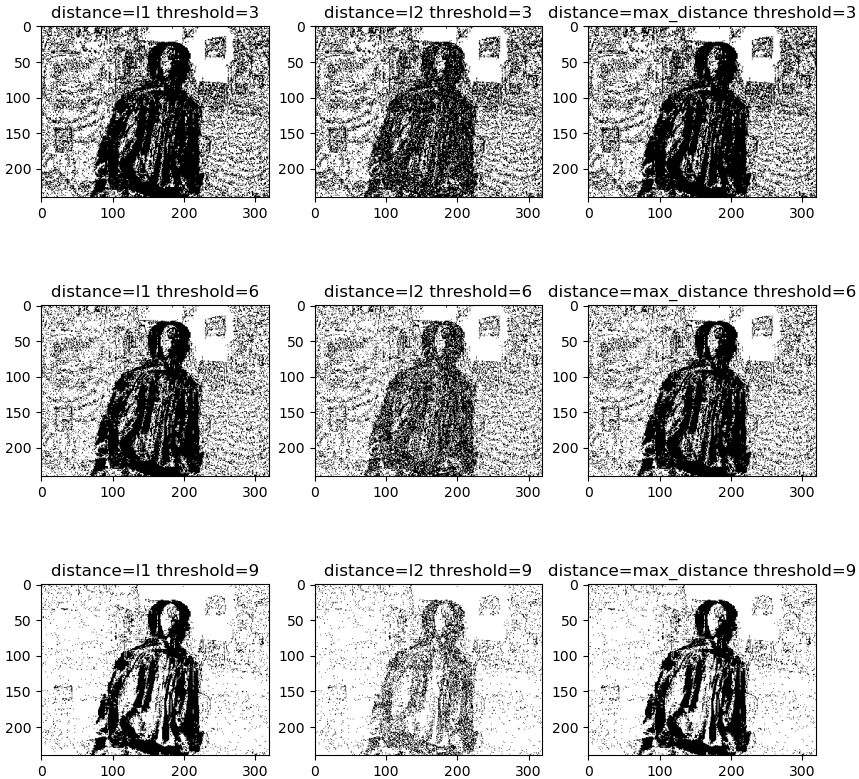
\includegraphics[width=200pt,height=200pt]{thr_distances.png}
    \caption{Threshold result on different distances}
    \label{fig:thr}
\end{figure}

\section{Detector}
The detector implemented is a simple Background Subtractor, as suggested.

The methodology used for creating the model was simply driven by trials and errors: thanks to the framework implemented I was able to add and remove operation to the pipeline and see the output in order to assert the correctness of it; in this way I built the pipeline and defined the parameters of each operation.

With a test pipeline\footnote{BackgroundNoGaussian class} was observed that the background subtractor (using the interpolated frame) was affected by artifact near the end of the video.

This happened with lower strength when Gaussian blur is used. \CREF{fig:gaussian}
\begin{figure}[ht]
    \centering
    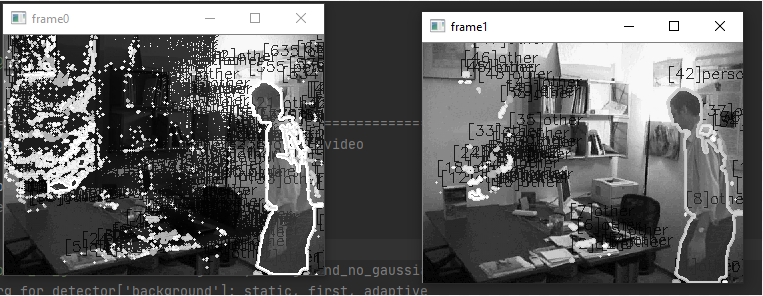
\includegraphics[width=0.5\textwidth,keepaspectratio]{background_no_gaussian.PNG}
    \caption{\textit{Pipeline} of BackgroundNoGaussian}
    \label{fig:gaussian}
\end{figure}

So in order to enhance the frame input a Gaussian blur is used for averaging pixels intensity without disrupting the image.

For removing noise, at the beginning, only opening with a filter of (9,9) was applied.
After some inconclusive trials in which the noise was not completely deleted I've tried the median filter, the "salt and pepper filter" which is used for impulse noise ( as the noisy pixels in a white-and-black image)
As we can see it perform better. \CREF{medfilter}

Moreover in order to remove additional noise the opening with a small filter is used afterwards.
\begin{figure}
    \centering
    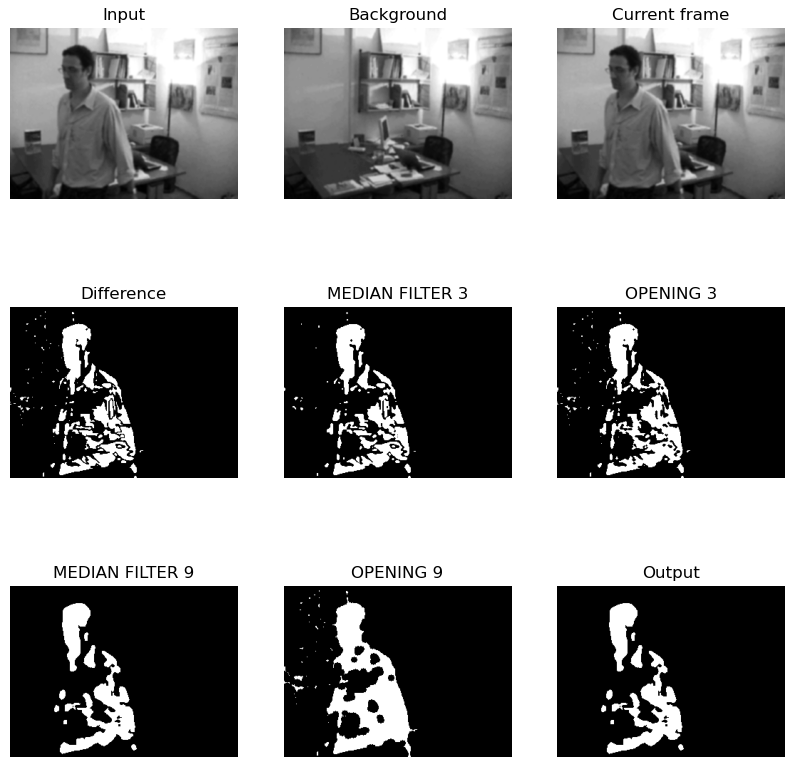
\includegraphics[width=0.4\textwidth,keepaspectratio]{median filter.png}
    \caption{Median filter and opening (ellipse kernel) using a kernel of size (3,3) and (9,9) }
    \label{medfilter}
\end{figure}


Based on the kind of background used:
    \begin{itemize}
        \item \textbf{static}: it was used as background the \textbf{frame 254}. \CREF{bg}
              \begin{figure}[ht]
                  \centering
                  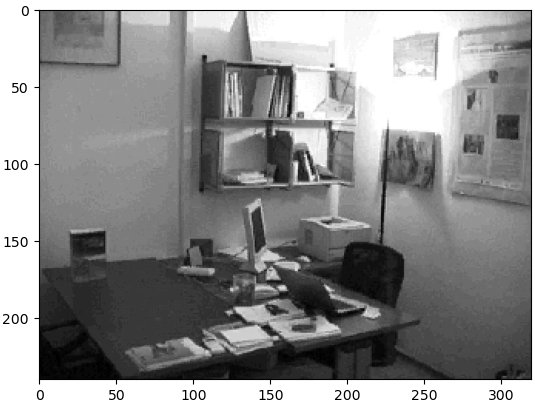
\includegraphics[width=0.5\textwidth,keepaspectratio]{bg.png}
                  \caption{Background image.\label{bg}}
              \end{figure}
        \item \textbf{first}: the background was interpolated using the first 100 frames.
        \item \textbf{adaptive}: the background is computed each time as the weighted average summation with the previous frame. Used for creating a detector without false positive.
    \end{itemize}  
different parameters and pipelines are defined.

The parameters are the following:

\begin{tabularx}{200pt}{c|ccc}
    kind     & distance      & threshold & alpha\footnote{alpha regulates the update speed (how fast the accumulator "forgets" about earlier images).} \\
    \hline
    static   & max\_distance & 30        & -     \\
    first    & max\_distance & 34        & -     \\
    adaptive & l1            & 5         & 0.70
\end{tabularx}

The pipelines are the following:

\begin{itemize}
    \item With testing was found that 34 was better for kind=first. \CREF{firstthr}
    \item Use alpha=0.70 in order to avoid to have detached blobs and so beeing able to reconstruct the blob with dilation. \CREF{adaptivealpha}
\end{itemize}


\begin{figure}
    \centering
    \begin{subfigure}[t]{0.45\textwidth}
        \centering
        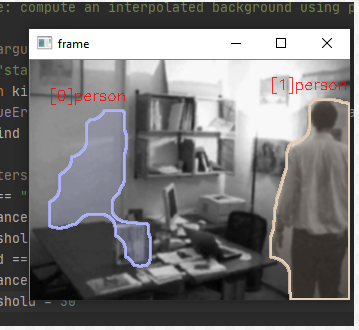
\includegraphics[width=120pt,keepaspectratio]{background_first_30.PNG}
        \caption{Using threshold=30}
    \end{subfigure}
    \begin{subfigure}[t]{0.45\textwidth}
        \centering
        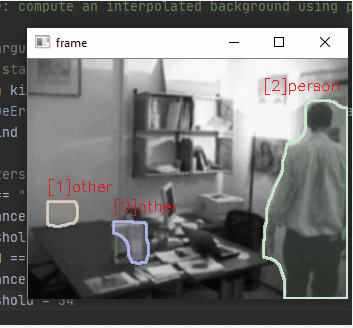
\includegraphics[width=120pt,keepaspectratio]{background_first_34.PNG}
        \caption{Using threshold=34}
    \end{subfigure}
    \caption{Background subtractor with kind=first}
    \label{firstthr}
\end{figure}

\begin{figure}
    \centering
    \begin{subfigure}[t]{0.45\textwidth}
        \centering
        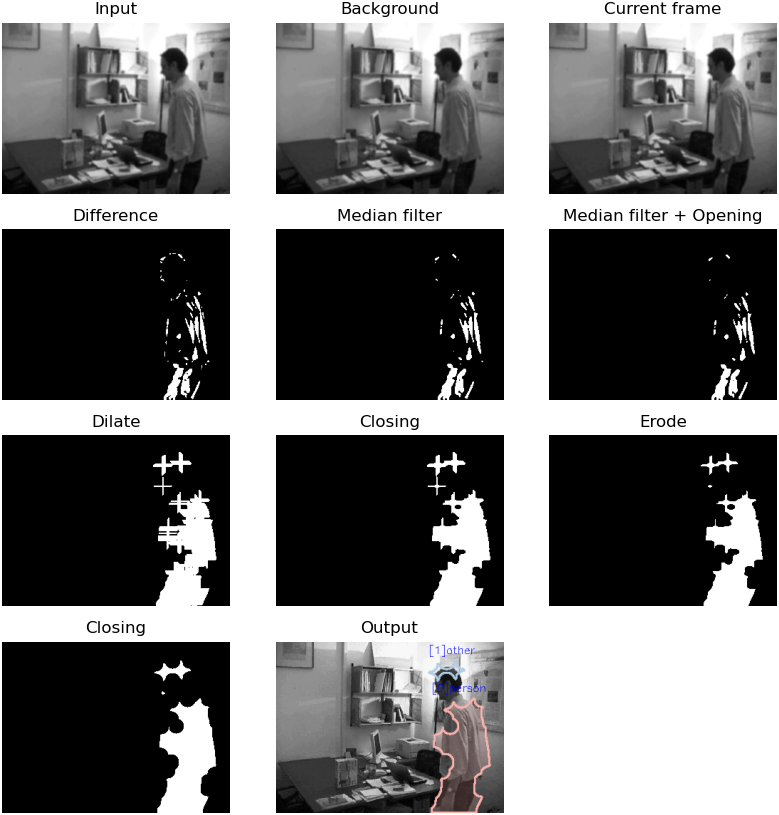
\includegraphics[width=160pt,keepaspectratio]{adaptive_alpha08_f482.png}
        \caption{Using alpha=0.8}
    \end{subfigure}
    \begin{subfigure}[t]{0.45\textwidth}
        \centering
        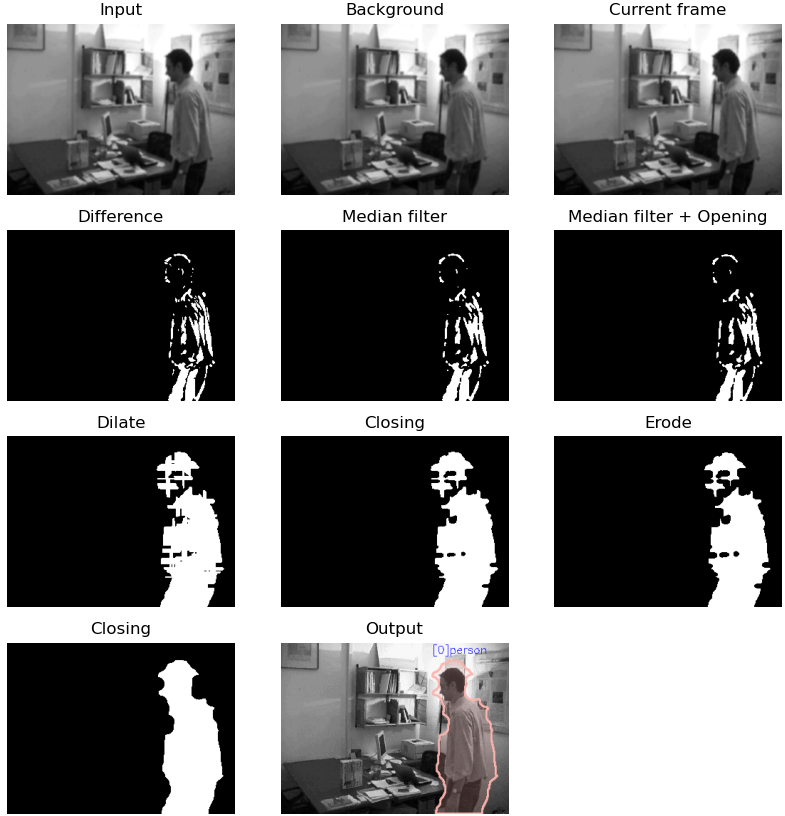
\includegraphics[width=160pt,keepaspectratio]{adaptive_alpha07_f482.png}
        \caption{Using alpha=0.7}
    \end{subfigure}
    \caption{Background subtractor with kind=adaptive}
    \label{adaptivealpha}
\end{figure}

After the noise is removed, a sequence of binary morphology operators is applied.

For kind=[\textbf{static},\textbf{first}]:
\begin{enumerate}
    \item Close horizontally using a rectangle filter
    \item Close vertically using a rectangle filter
    \item Dilate for filling the void
    \item Closing for filling the holes
\end{enumerate}
For kind=\textbf{adaptive} a more aggressive pipeline is used:
\begin{enumerate}
    \item Dilate for filling the void caused by median filter using a cross filter with a size = (20,20)
    \item Two closing with an elliptical kernel with size (5,5) and (20,20) separated by an erode operation in order to reduce the boundaries of the blobs.
\end{enumerate}

I have also tried to improve the contour detection using Canny edge detection algorithm (using the new detected edges for refining the already found edges) but was impossible to filter out noisy information from it using binary morphology operators. \CREF{canny}

\begin{figure}
    \centering
    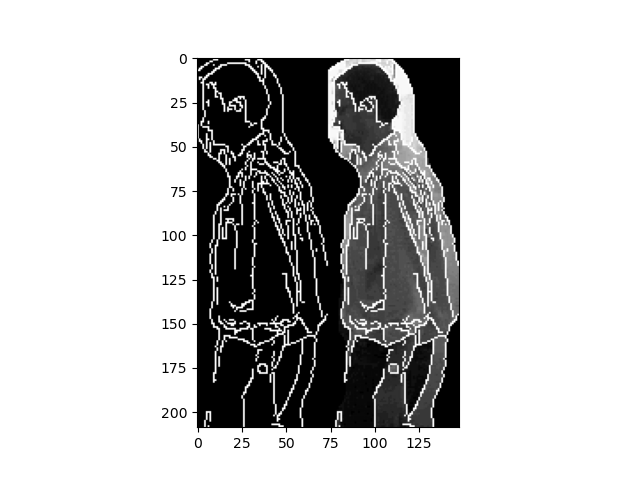
\includegraphics[width=0.5\textwidth,keepaspectratio]{canny.png}
    \caption{Canny edge detection algorithm applied to the inner area of the contour. Left: edges computed using Canny. Right: Edges overlapped on the image. Any binary morphology operator is going to remove also the edges.}
    \label{canny}
\end{figure}

\section{Filtering}
The information read about the contours are : area, perimeter, ratio, rectangularity, circularity, mean and standard deviation (in this case mean and standard deviation of the image inside the bounding box of the contour).



For filtering contours, first it is done a check on rectangularity and then on the area and perimeter.
This three information were chosen after reasoning on top of the logs produced by the detector.

I was thinking to use circularity, also, to filter out perfect circle but I have observed that sometimes blobs with high rectangularity have high circularity: the idea was to filter out isolated point that are enlarged by dilation.

\clearpage
\section{Handling false positive}
In order to detect false positives two solutions are proposed:
\begin{itemize}
    \item Compute the standard deviation of the image, normalized over 255, after computing its gradient: I think that using the raw image could be misleading.

    The image used is the one inside the bounding box because of misleading edges found using the inner area. \CREF{grad}


    In this case the contour segment is still in the image but is labeled as false positive. \CREF{Figure:fpl}

    Reasoning only on top of the contour is not possible because the segmentation doesn't return always the exact contour.

    The \textbf{threshold} used for detecting \textbf{false positive} is \textbf{$0.1$} chosen after reding the logs.

    \item Compute the background as an weighted sum with the previous frame at each time step. In this case the object is not detected; moreover also the other object, which is steady after beeing moved by the human, is ignored. \CREF{Figure:fpi}
\end{itemize}

\begin{figure}
    \centering
    \begin{minipage}{0.3\textwidth}
        \centering
        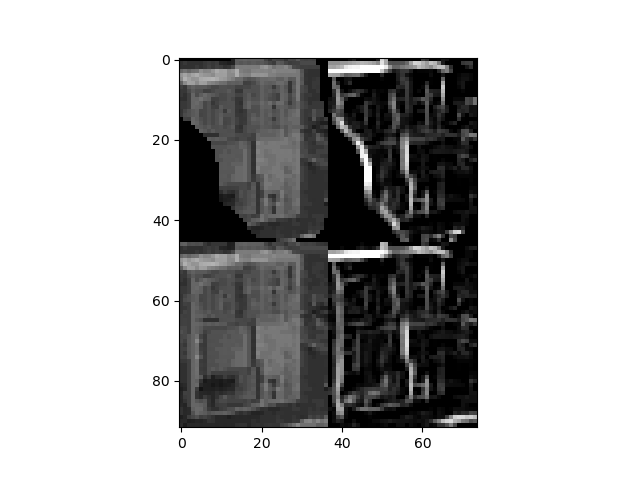
\includegraphics[width=\linewidth]{grad1.png}
        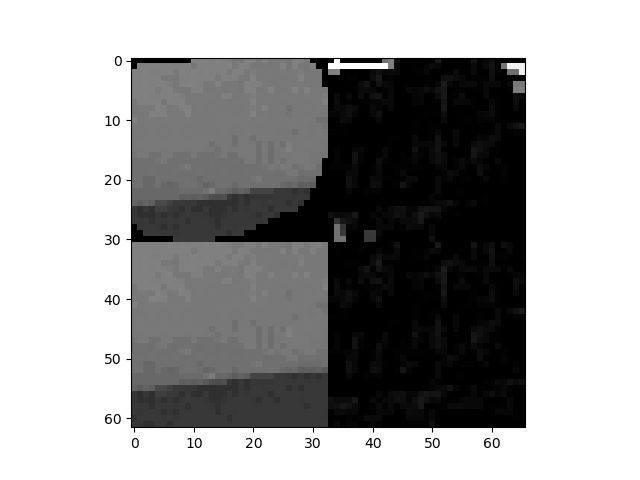
\includegraphics[width=\linewidth]{grad2.png}
    \end{minipage}%
    \begin{minipage}{0.7\textwidth}
        \centering
        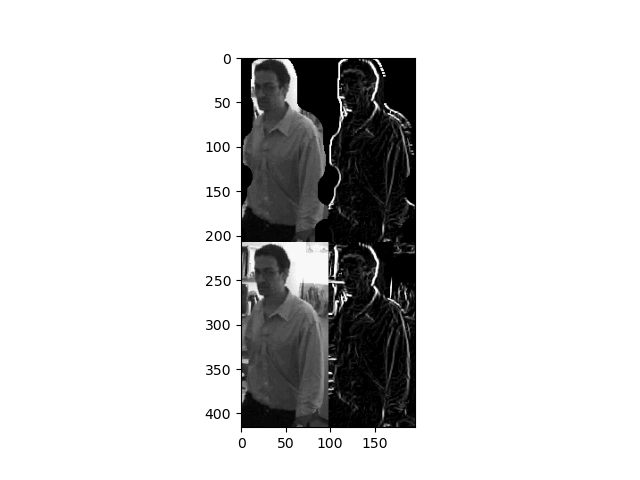
\includegraphics[scale=0.6]{grad3.png}
    \end{minipage}

    \caption{Gradient computed for each blob. Top: using the inner area. Bottom: using the bounding box.}
    \label{grad}
\end{figure}

\begin{figure}[ht]
    \centering
    \begin{subfigure}{0.47\textwidth}
        \centering
        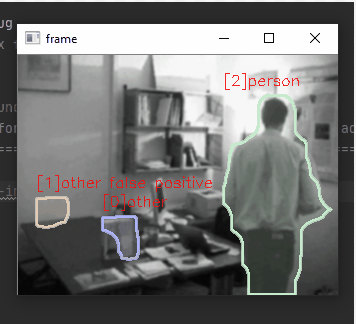
\includegraphics[width=150pt,keepaspectratio]{background_static_falsepositive.PNG}
        \caption{Using kind=[static,first].}
        \label{Figure:fpl}
    \end{subfigure}
    \begin{subfigure}{0.47\textwidth}
        \centering
        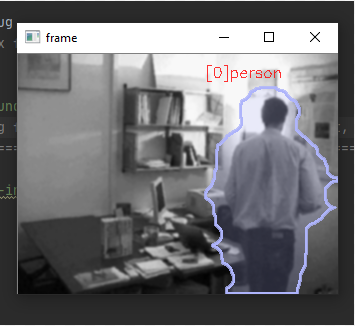
\includegraphics[width=150pt,keepaspectratio]{background_adaptive_falsepositive.PNG}
        \caption{Using kind=adaptive.}
        \label{Figure:fpi}
    \end{subfigure}
    \caption{False positive detection}
\end{figure}

\section{Conclusion}
The performance, measured as how much the pipeline is able to capture the human silhouette, are similar between using a static background and an interpolated one since the use the same pipeline instead the adaptive one is worse but although it is able to avoid false positive. \CREF{out481}

\begin{figure}
    \begin{subfigure}{0.3\textwidth}
        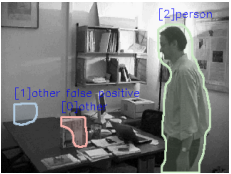
\includegraphics[width=\linewidth,keepaspectratio]{out481_static.PNG}
        \caption{Using kind=static}
    \end{subfigure}
    \begin{subfigure}{0.3\textwidth}
        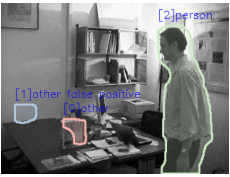
\includegraphics[width=\linewidth,keepaspectratio]{out481_first.PNG}
        \caption{Using kind=first}
    \end{subfigure}
    \begin{subfigure}{0.3\textwidth}
        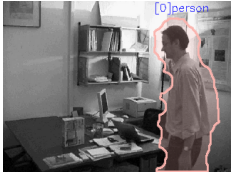
\includegraphics[width=\linewidth,keepaspectratio]{out481_adaptive.PNG}
        \caption{Using kind=adaptive}
    \end{subfigure}
    \caption{Output of the frame 481.}
    \label{out481}
\end{figure}
\end{document}

